\documentclass[a4paper]{article}

%use the english line for english reports
%usepackage[english]{babel}
\usepackage[portuguese]{babel}
\usepackage[utf8]{inputenc}
\usepackage{indentfirst}
\usepackage{graphicx}
\usepackage{verbatim}
\usepackage{listings}
\usepackage{mathtools}


\begin{document}

\setlength{\textwidth}{16cm}
\setlength{\textheight}{22cm}

\title{\Huge\textbf{Syrtis}\linebreak\linebreak\linebreak
\Large\textbf{Relatório Final}\linebreak\linebreak
\linebreak\linebreak

\includegraphics[scale=0.1]{feup-logo.png}\linebreak\linebreak
\linebreak\linebreak
\Large{Mestrado Integrado em Engenharia Informática e Computação} \linebreak\linebreak
\Large{Programação em Lógica}\linebreak
}

\author{\textbf{Grupo 79:}\\
Flávio Couto - 201303726 \\
Pedro Afonso Castro - 201304205 \\
\linebreak\linebreak \\
 \\ Faculdade de Engenharia da Universidade do Porto \\ Rua Roberto Frias, s\/n, 4200-465 Porto, Portugal \linebreak\linebreak\linebreak
\linebreak\linebreak\vspace{1cm}}
%\date{Junho de 2007}
\maketitle
\thispagestyle{empty}

%************************************************************************************************
%************************************************************************************************

\newpage

\section*{Resumo}

Para a unidade curricular de Programação em Lógica, o grupo comprometeu-se a desenvolver na linguagem PROLOG o jogo Syrtis, um jogo de estratégia cujo objetivo é criar uma ilha com todas as peças da nossa cor ou forma, impedindo que o adversário faça o mesmo com as suas.

O objetivo deste projeto foi colocarmos em prática os assuntos abordados nas aulas, bem como compreender um paradigma de programação no qual não tínhamos ainda qualquer experiência. Para tal, fizemos pesquisa, estudo e planeamento, de forma a podermos cumprir não só os objetivos propostos pelos professores, como também os nossos objetivos de aprofundar os nossos conhecimentos acerca de um novo paradigma de programação. Como resultado, ficámos com um jogo, executável em linha de comandos, bastante interessante e robusto, que nos orgulhamos de ter realizado.

Para concluir, entendemos que fomos capazes de cumprir com os objetivos propostos, tanto pelos professores, visto que conseguimos desenvolver todos os objetivos propostos, como por nós, porque conseguimos não só consolidar os conhecimentos aprendidos nas aulas, bem como aprofundar os nossos conhecimentos acerca do PROLOG.
\newpage

\tableofcontents

%************************************************************************************************
%************************************************************************************************

%*************************************************************************************************
%************************************************************************************************

\newpage

%%%%%%%%%%%%%%%%%%%%%%%%%%
\section{Introdução}

O principal objetivo deste projeto é adquirir competências ao nível da Programação em Lógica através do estudo de um jogo de tabuleiro previamente escolhido. Foram-nos dadas várias hipóteses de jogos, tendo nós escolhido o Syrtis, por causa da sua elevada componente estratégica e tática, bem como alguma complexidade, sempre necessária para trazer um maior sentimento de desafio quando nos é colocado um projeto em mãos.

Este relatório contém várias secções. Uma secção a descrever as história e regras do jogo, com imagens para ajudar à sua compreensão, outra secção com a descrição da lógica utilizada para a implementação do jogo, nomeadamente a sua visualização, execução de movimentos, verificação do cumprimento das regras do jogo, teste da condição de vitória e a inteligência artificial do computador quando o utilizador escolhe jogar em modo \textit{single player}, uma descrição da interface com o utilizador, em modo textual, uma conclusão acerca dos objetivos cumpridos e por cumprir, uma lista de fontes utilizadas para a produção deste relatório e do código-fonte, e por último uma série de elementos anexados, nomeadamente o código fonte do projeto.

%%%%%%%%%%%%%%%%%%%%%%%%%%
\section{O Jogo Syrtis}

Segue-se uma explicação das regras do Syrtis, bem como alguns exemplos para melhor demonstrar alguns aspetos que possam ser de maior dificuldade de compreensão.

\subsection{História}

	O Syris é um jogo de estratégia em que os dois jogadores se encontram numa ilha instável e desconhecida. A paisagem da ilha está sempre em mudança, e o avanço do mar faz com que a ilha esteja a tornar-se cada vez mais pequena... Para complicar ainda mais, este avanço está a fazer com que se formem areias movediças, limitando ainda mais o espaço habitável na ilha... Apenas um dos jogadores poderá sobreviver, quem será capaz de ser o mais forte?
	
\subsection{Objetivo}
	
	A cada jogador é atribuída uma forma e uma cor (quadrado e preto ou círculo e branco). O objetivo do jogo é conquistar todas as peças que contenham a sua cor ou a sua forma.
	
\subsection{Equipamento}

	O jogo é composto por peças quadradas com uma determinada forma e cor. Há 4 combinações possíveis: círculos e quadrados brancos e pretos. Há também quatro torres, duas brancas e circulares e duas pretas e quadradas.
	
\subsection{Preparação}

	As peças quadradas são inicialmente aleatoriamente dispostas num de dois formatos de ilha. Para um jogo mais longo e estratégico, utiliza-se o formato Syrtis Major. Para um jogo mais curto e tático, utiliza-se o formato Syrtis Minor. As figuras \ref{fig:syrtismajor} e \ref{fig:syrtisminor} mostram a estrutura destes dois formatos.
	
\begin{figure}[h]

\begin{minipage}{0.5\linewidth}
\centering
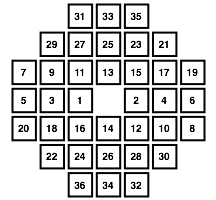
\includegraphics[scale=0.9]{syrtismajor.png}
\caption{Syrtis Major}
\label{fig:syrtismajor}
\end{minipage}
\quad
\begin{minipage}{0.5\linewidth}
\centering
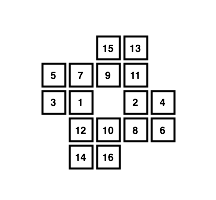
\includegraphics[scale=0.9]{syrtisminor.png}
\caption{Syrtis Minor}
\label{fig:syrtisminor}
\end{minipage}

\end{figure}

Depois, um dos jogadores coloca as 4 torres por cima de uma das peças à sua escolha, desde que sejam da cor ou da forma dessa peça. O outro jogador decide se quer jogar com as torres brancas circulares ou pretas quadradas e o jogo começa por quem tiver ficado com as peças brancas e circulares.

\subsection{Ilhas}

Uma ilha é uma peça ou um grupo de peças que partilham a mesma forma ou cor. Para serem consideradas uma ilha, devem estar adjacentes horizontal ou verticalmente. Há quatro tipos de ilhas: ilhas pretas, brancas, quadradas e circulares. Uma peça pode obviamente pertencer a uma ilha de uma cor e a uma ilha de uma forma ao mesmo tempo. As figuras \ref{fig:circleisland} e \ref{fig:blackisland} mostram exemplos de ilhas.

\begin{figure}[h]

\begin{minipage}{0.5\linewidth}
\centering
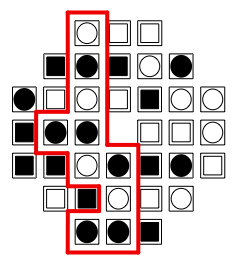
\includegraphics[scale=0.75]{island1.png}
\caption{Ilha de círculos}
\label{fig:circleisland}
\end{minipage}
\quad
\begin{minipage}{0.5\linewidth}
\centering
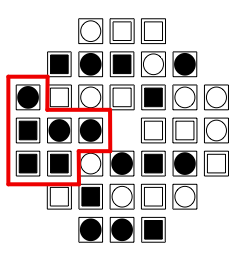
\includegraphics[scale=0.75]{island2.png}
\caption{Ilha de pretos}
\label{fig:blackisland}
\end{minipage}

\end{figure}


\subsection{Acções}
\label{sec:actions}

Em cada turno cada jogador pode fazer uma de entre 4 acções possíveis: mover uma torre, afundar uma peça, deslocar uma peça, ou passar a sua vez.

\subsubsection{Mover uma torre}

Cada jogador pode mover uma das suas torres, desde que se mantenha em pelo menos uma das suas duas ilhas atuais (ou seja, ou na ilha respeitante à forma ou na ilha respeitante à cor). As outras torres não bloqueiam este movimento, ou seja, podemos passar por cima de outras torres.  A figura \ref{fig:towermovement} mostra um exemplo do movimento de uma torre.

\begin{figure}[h]
\centering
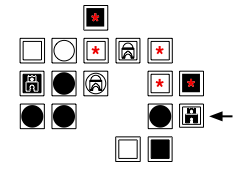
\includegraphics[scale=0.9]{towermovement.png}
\caption{Movimento de uma torre}
\label{fig:towermovement}
\end{figure}

A torre indicada (preta e quadrada) pode mover-se para qualquer uma das peças marcadas com uma seta, pois estas encontram-se na sua ilha quadrangular. Note-se também que ela não pode ir para a peça à sua esquerda, visto que, apesar de ser preta, esta não se encontra na sua ilha (visto que a peça em que a torre se encontra é branca e quadrada, e a peça em questão é preta e circular).

\subsubsection{Afundar uma peça}

Cada jogador pode remover uma peça do tabuleiro se:

\begin{itemize}
\item Esta for adjacente a uma peça ocupada por uma torre desse jogador;
\item Esta estiver desocupada;
\item Esta tiver pelo menos um espaço adjacente livre.
\end{itemize}

A figura \ref{fig:sinktile} mostra um exemplo de quais peças podem ser afundadas.

\begin{figure}[h]
\centering
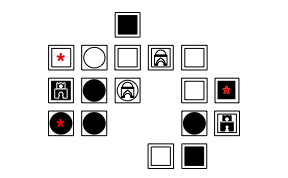
\includegraphics[scale=0.9]{sinktile.png}
\caption{Peças afundáveis}
\label{fig:sinktile}
\end{figure}


O jogador preto pode afundar quaisquer peças que estejam marcadas com uma estrela. Nenhuma peça branca está numa posição que lhe permita afundar alguma peça.

\subsubsection{Deslocar uma peça}

Um jogador poderá deslocar uma peça ocupada por uma das suas torres através de quaisquer espaços vazios que estejam conectados. A peça pode ser movida em qualquer direcção, quantas vezes quisermos, desde que a largura ou altura do tabuleiro não seja aumentada (nem mesmo a meio do movimento) e as peças do tabuleiro continuem conectadas. A figura \ref{fig:slidetile} mostra um exemplo disto.

\begin{figure}[h]
\centering
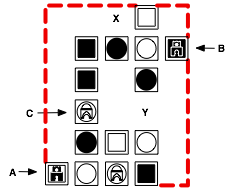
\includegraphics[scale=0.9]{slidetile.png}
\caption{Peças deslocáveis}
\label{fig:slidetile}
\end{figure}

A torre A pode mover a sua peça para a posição X, mas a torre B não pode (visto que teria de aumentar o tamanho do tabuleiro a meio da jogada para o fazer). A torre C apenas se pode deslocar para a posição Y, porque é a unica posição em que o tabuleiro continua todo conectado. A outra torre não se pode mexer.

\subsubsection{Passar a vez}

Basta não fazer nada e passar a vez ao outro jogador. Um jogador que não pode fazer nada é obrigado a passar.


\subsection{Fim do jogo}
\label{endgame}

Há três formas de ganhar o jogo. Uma já foi dita anteriormente (ter uma ilha completa). As outras duas são usadas principalmente para evitar empates e que os jogos durem demasiado tempo.

\subsubsection{Ilha completa}

Um jogador vence quando todas as peças restantes da sua cor, ou da sua forma, estão conectadas.
Se todas as peças de\begin{figure}[h]
\centering
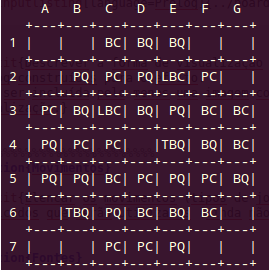
\includegraphics[scale=0.5]{outputboard.png}
\caption{Output produzido no terminal para o tabuleiro}
\label{fig:outputboard}
\end{figure} uma cor ou forma estão conectadas quando o tabuleiro é inicialmente construído, o jogador que colocar as torres deve inicalmente trocar duas peças cuja numeração no formato de jogo usado (ver figuras \ref{fig:syrtismajor} e \ref{fig:syrtisminor}) sejam seguidas. Por exemplo, trocar a peça 11 com a peça 12. Deve continuar a usar-se este método até que tal deixe de acontecer.

\subsubsection{Areias movediças}

Se um jogador afundar quatro peças sem o outro jogador ter afundado nenhuma, o segundo perde, sendo engolido pelas areias movediças.
Os jogadores devem controlar quantas peças afundaram desde que o outro jogador afundou a última peça.

\subsubsection{Iniciativa}

Esta regra existe para evitar empates. O jogo termina se alguma das seguintes situações ocorrer:

\begin{itemize}
\item Ambos os jogadores conseguem uma ilha completa ao mesmo tempo;
\item Ambos os jogadores passam a sua vez em jogadas consecutivas (ou seja, ambos passam duas vezes cada um);
\item Um jogador passa quatro vezes seguidas.
\end{itemize}

Em qualquer um dos casos, o último jogador a afundar uma peça ganha. Se nenhum dos jogadores tiver afundado uma peça, o jogador que jogou primeiro ganha.

\begin{figure}[h]
\centering
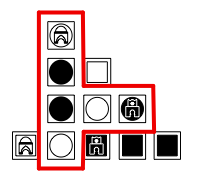
\includegraphics[scale=0.9]{win.png}
\caption{Uma situação em que o jogador branco ganhou ao completar uma ilha de círculos.}
\label{fig:win}
\end{figure}


%%%%%%%%%%%%%%%%%%%%%%%%%%
\section{Lógica do Jogo}

\subsection{Representação do Estado do Jogo}
\label{gamestate}

O estado do jogo é guardado recorrendo à base de dados do PROLOG. Cada peça é guardada sob a forma de um predicado, utilizando o formato [Torre,Cor,Forma].

\begin{itemize}
\item \textbf{Torre:} Representa a existência ou não de uma torre no quadrado. Em caso afirmativo, utiliza a letra 'L' para representar uma torre branca, circular, e uma letra 'T' para uma torre preta, quadrangular.
\item \textbf{Cor:} Representa a cor da do quadrado. Se for preto, utiliza-se a letra 'P', se for branco utiliza-se a letra 'B'.
\item \textbf{Forma:} Representa a forma da peça do quadrado. Se for um círculo, usa-se a letra 'C', se for um quadrado usa-se a letra 'Q'.
\end{itemize}

Para todos os casos, a não existência do objeto implica a representação através de um espaço (' ').

Segue-se um exemplo de representação do board quando o jogo começa:

\begin{lstlisting}
beggining_board(Board) :- Board =
[	[[' ',' ',' '], [' ',' ',' '],[' ','B','C'], [' ','B','Q'],
	 [' ','B','Q'], [' ',' ',' '],[' ',' ',' ']],
	[[' ',' ',' '], [' ','P','Q'],[' ','P','C'], [' ','P','Q'],
 	 ['L','B','C'], [' ','P','C'], [' ',' ',' ']],
	[[' ','P','C'], [' ','B','Q'], ['L','B','C'], [' ','B','Q'],
	 [' ','P','Q'], [' ','B','C'], [' ','B','C']],
	[[' ','P','Q'], [' ','P','C'], [' ','P','C'], [' ',' ',' '],
	 ['T','B','Q'], [' ','B','Q'], [' ','B','C']],
 	[[' ','P','Q'], [' ','P','Q'], [' ','B','C'], [' ','P','C'],
 	 [' ','P','Q'], [' ','P','C'], [' ','B','Q']],
 	[[' ',' ',' '], ['T','B','Q'], [' ','P','Q'], [' ','B','C'],
 	 [' ','B','Q'], \begin{figure}[h]
\centering
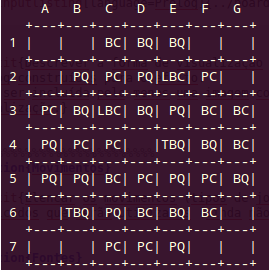
\includegraphics[scale=0.5]{outputboard.png}
\caption{Output produzido no terminal para o tabuleiro}
\label{fig:outputboard}
\end{figure}[' ','B','C'], [' ',' ',' ']],
 	[[' ',' ',' '], [' ',' ',' '], [' ','P','C'], [' ','P','C'],
 	 [' ','P','Q'], [' ',' ',' '], [' ',' ',' ']]].
\end{lstlisting}

Quando o jogo está a meio:

\begin{lstlisting}
middle_board(Board) :- Board =
[	[[' ',' ',' '], [' ',' ',' '], [' ',' ',' '], [' ',' ',' '],
	 [' ','B','Q'], [' ',' ',' '], [' ',' ',' ']],
 	[[' ',' ',' '], [' ',' ',' '], [' ','P','Q'], [' ','P','C'],
 	 [' ','B','C'], ['T','P','Q'], [' ',' ',' ']],
	[[' ',' ',' '], [' ',' ',' '], [' ','P','Q'], [' ',' ',' '],
	 [' ','P','Q'], [' ',' ',' '], [' ',' ',' ']],
	[[' ',' ',' '], [' ',' ',' '], ['L','B','C'], [' ',' ',' '],
	 [' ',' ',' '], [' ',' ',' '], [' ',' ',' ']],
 	[[' ',' ',' '], [' ',' ',' '], [' ','P','C'], [' ','B','Q'],
 	 [' ',' ',' '], [' ',' ',' '], [' ',' ',' ']],
 	[[' ',' ',' '], ['T','B','Q'], [' ','B','C'], ['L','B','C'],
 	 [' ','P','Q'], [' ',' ',' '], [' ',' ',' ']],
 	[[' ',' ',' '], [' ',' ',' '], [' ',' ',' '], [' ',' ',' '],
 	 [' ',' ',' '], [' ',' ',' '], [' ',' ',' ']]].
\end{lstlisting}

E quando o jogo acaba:

\begin{lstlisting}
end_board(Board) :- Board =
[	[[' ',' ',' '], [' ',' ',' '], [' ',' ',' '], [' ',' ',' '],
	 [' ',' ',' '], [' ',' ',' '], [' ',' ',' ']],
 	[[' ',' ',' '], [' ',' ',' '], [' ',' ',' '], [' ',' ',' '],
 	 [' ',' ',' '], [' ',' ',' '], [' ',' ',' ']],
	[[' ',' ',' '], \begin{figure}[h]
\centering
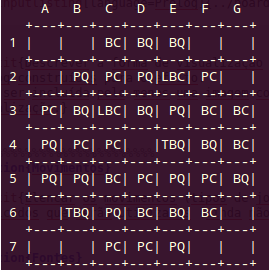
\includegraphics[scale=0.5]{outputboard.png}
\caption{Output produzido no terminal para o tabuleiro}
\label{fig:outputboard}
\end{figure}[' ',' ',' '], ['L','B','C'], [' ',' ',' '],
	 [' ',' ',' '], [' ',' ',' '], [' ',' ',' ']],
	[[' ',' ',' '], [' ',' ',' '], [' ','P','C'], [' ','Q','B'],
	 [' ',' ',' '], \begin{figure}[h]
\centering
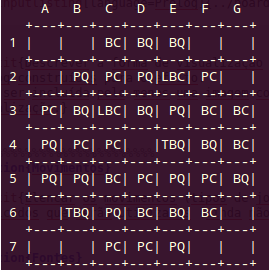
\includegraphics[scale=0.5]{outputboard.png}
\caption{Output produzido no terminal para o tabuleiro}
\label{fig:outputboard}
\end{figure}[' ',' ',' '], [' ',' ',' ']],
 	[[' ',' ',' '], [' ',' ',' '], [' ','P','C'], [' ','B','C'],
 	 ['T','B','C'], [' ',' ',' '], [' ',' ',' ']],
 	[['L','B','Q'], [' ','B','C'], ['T','P','Q'], [' ','P','Q'],
 	 [' ','P','Q'], [' ',' ',' '], [' ',' ',' ']],
 	[[' ',' ',' '], [' ',' ',' '], [' ',' ',' '], [' ',' ',' '],
 	 [' ',' ',' '], [' ',' ',' '], [' ',' ',' ']]].
\end{lstlisting}

Para além do tabuleiro, outros aspetos importantes para a representação do estado de jogo, como o jogador que está atualmente a jogar, ou quem tem a sequência de peças afundadas atual, são também guardadas na base de dados do PROLOG.

\subsection{Visualização do Tabuleiro}

O tabuleiro é gerado aleatoriamente, começando por se inicializar os predicados na base de dados recorrendo ao seguinte predicado:

\begin{lstlisting}
create_database(+Length).
\end{lstlisting}

Em que Length é o tamanho do tabuleiro, que terá o tamanho 5 se for um tabuleiro do tipo Syrtis Minor ou 7 se for um do tipo Syrtis Major. Depois disso, as peças são colocadas de forma aleatória, sendo chamadas um dos seguintes predicados consoante do tipo de tabuleiro:

\begin{lstlisting}
randomize_board_major.
\end{lstlisting}

ou 

\begin{lstlisting}
randomize_board_minor.
\end{lstlisting}

Tal como foi referido na secção \ref{gamestate}, nós recorremos à base de dados do PROLOG para guardar o estado do tabuleiro, pelo que não se torna necessário retornar informação nenhuma acerca deste.

A figura \ref{fig:outputboard} mostra uma imagem com o output produzido.

\begin{figure}[h]
\centering
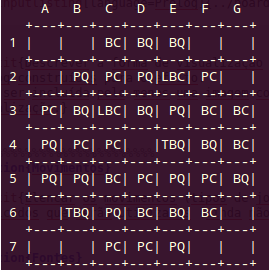
\includegraphics[scale=0.5]{outputboard.png}
\caption{Output produzido no terminal para o tabuleiro}
\label{fig:outputboard}
\end{figure}

\subsection{Lista de Jogadas Válidas}

Para se obter uma lista de jogadas válidas para cada jogador, recorre-se ao seguinte predicado:

\begin{lstlisting}
available_actions(+Player, -Actions).
\end{lstlisting}

Em Actions é retornada uma lista de listas, cada lista contendo informação acerca do tipo de jogada (Afundar uma peça, mover uma peça, mover uma torre ou passar a vez), bem como as coordenadas necessárias para cada tipo de jogada.

\subsection{Execução de Jogadas}

Em cada jogada, é pedido ao jogador para decidir qual a jogada, de entre as 4 possíveis, que pretende fazer, bem como as coordenadas necessárias para fazer a jogada. Cada uma destas jogadas passa por um processo de validação, que, dependendo do tipo de jogada, passa por um destes 3 predicados:

\begin{lstlisting}
valid_slide(+X,+Y,+NX,+NY).
valid_sink(+X,+Y).
valid_move(+X,+Y,+NX,+NY).
\end{lstlisting}

Passar a vez não envolve qualquer tipo de verificação. Caso o predicado falhe, o \textit{backtracking} do PROLOG levará a que seja apresentado ao jogador a mensagem inicial de escolher uma jogada, fazendo com que este possa tentar outra vez, sucessivamente, até fazer uma jogada válida.

A figura \ref{fig:makeplay} mostra um exemplo de um jogador a realizar uma jogada.

\begin{figure}[h]
\centering
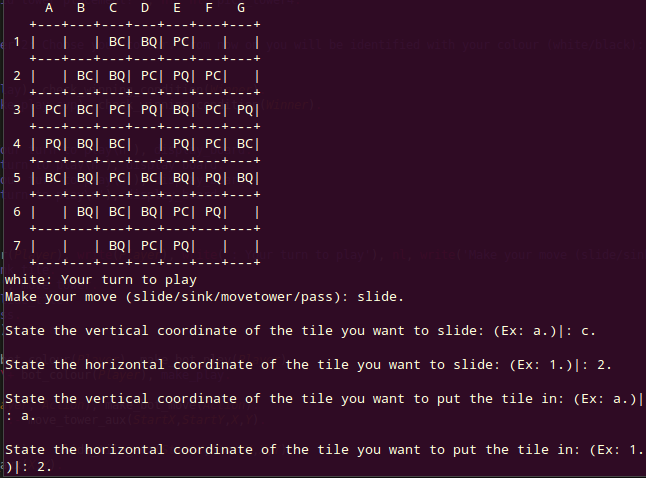
\includegraphics[scale=0.5]{makeplay.png}
\caption{Exemplo de uma jogada.}
\label{fig:makeplay}
\end{figure}

\subsection{Avaliação do Tabuleiro}
\label{boardeval}
A avaliação do tabuleiro é feita recorrendo ao seguinte predicado:

\begin{lstlisting}
evaluate_board(+Player, -Score).
\end{lstlisting}

Esta avaliação é feita recorrendo a uma função de avaliação, que utiliza os seguintes critérios:

\subsubsection{Critério do número de peças}

Este critério baseia-se no facto de que quanto mais peças da nossa cor/forma e quanto menos peças da cor/forma do adversário há no tabuleiro, melhor. O cálculo deste critério é feito recorrendo à seguinte formula:

\begin{equation*}
\begin{multlined}
Resultado = numPecasCorBot + numPecasFormaBot - \\
(numPecasCorJogador + numPecasFormaJogador)
\end{multlined}
\end{equation*}

\subsubsection{Critério da proximidade ao centro}

Este critério baseia-se no facto de que quanto mais próxima uma peça está do centro, mais valiosa é, ou seja, devemos dar prioridade a manter as nossas peças no centro, enquanto afundamos as peças do adversário que estejam mais próximas do centro. Infelizmente este é um critério muito pesado computacionalmente, visto que envolve uma elevada quantidade de cálculos, pelo que restringimos esta avaliação apenas às peças que é possível afundar tendo em conta o estado atual do jogo. O cálculo deste critério é feito recorrendo à seguinte fórmula:

\begin{equation*}
\begin{multlined}
Resultado = \sum\limits_{i=1}^{pBot} 10 * ((MaxDist - Dist) / MaxDist) - \\\sum\limits_{i=1}^{pJog} 10 * ((MaxDist - Dist) / MaxDist)
\end{multlined}
\end{equation*}

Em que \textit{pBot} e \textit{pJog} representam as peças do Bot e do Jogador, respetivamente, \textit{MaxDist} a distância máxima possível de uma peça ao centro e \textit{Dist} a distância da peça ao centro.

\subsubsection{Critério das ilhas}

Este critério baseia-se no facto de que quanto mais peças tiver uma ilha em relação ao número total das peças do tipo dessa ilha, mais perto estamos de ganhar o jogo e, consequentemente, o tabuleiro tem mais valor. Mais uma vez, por este também ser um critério pesado computacionalmente, restringimos este cálculo apenas às ilhas onde se encontram as quatro torres. A fórmula para o cálculo deste critério é a seguinte:

\begin{equation*}
\begin{multlined}
Resultado = 50 * ((TamIlhaCorBot1 + TamIlhaCorBot2) / NCorBot) + \\ ((TamIlhaFormaBot1 + TamIlhaFormaBot2) / NFormaBot) - \\
					( ((TamIlhaCorJog1 + TamIlhaCorJog2) / NCorJog) + \\ ((TamIlhaFormaJog1 + TamIlhaFormaJog2) / NFormaJog) )
\end{multlined}
\end{equation*}

Os números 1 e 2 representam as torres 1 e 2 de cada jogador.

\subsubsection{Critério da sequência de peças afundadas}

Este critério baseia-se no facto de que quanto maior estiver uma sequência de peças afundadas para um jogador, mais valioso está o tabuleiro para esse jogador, já que se um jogador afundar 4 peças sem o outro afundar nenhuma, esse jogador ganha o jogo. A fórmula para o cálculo deste critério é a seguinte:

Se o bot estiver com a sequência atual:
\begin{equation*}
\begin{multlined}
Resultado = 20 * NPecasAfundadas
\end{multlined}
\end{equation*}

Se o jogador estiver com a sequência atual:

\begin{equation*}
\begin{multlined}
Resultado = -20 * NPecasAfundadas
\end{multlined}
\end{equation*}

\subsubsection{Critério de vitória}

Este critério testa se alguma jogada leva a alguma condição de vitória, e se encontrar alguma, atribui um valor de 10000 a essa jogada, fazendo com que seja sempre a jogada escolhida. No caso em que alguma jogada leve à vitória do jogador, atribui-lhe um valor de -10000.

\subsection{Final do Jogo}

Sempre que o ciclo de jogo é executado, o programa testa se alguma das condições de vitória foi atingida, chamando o predicado

\begin{lstlisting}
check_winning_condition(-Winner)
\end{lstlisting}

Se este predicado suceder, então o vencedor estará em Winner. Caso contrário, o ciclo continua. Este predicado testa as 3 condições de vitória descritas na secção  \ref{endgame}. 

\subsection{Jogada do Computador}

O computador tem dois modos possíveis de funcionamento: um modo fácil e um modo difícil. No modo fácil, ele simplesmente escolhe uma jogada aleatoriamente, não se preocupando se a jogada é prejudicial ou não. No modo difícil, o computador avalia os critérios descritos na secção \ref{boardeval} para cada jogada possível, e escolhe a jogada que lhe permite obter um tabuleiro mais benéfico. Tendo em conta a complexidade do nosso jogo, tornou-se impossível ir além de uma avaliação ao estado atual do tabuleiro, visto que isso significaria que o cálculo demoraria demasiado tempo e não seria feito em tempo útil.

O predicado que determina a jogada do computador é o seguinte:

\begin{lstlisting}
bot_action(+Difficulty, +Player, -Action).
\end{lstlisting}

Em que Difficulty é 0 se for o modo fácil e 1 se for o modo difícil, player é a cor do bot e Action a acção determinada.

%%%%%%%%%%%%%%%%%%%%%%%%%%
\section{Interface com o Utilizador}

A interface com o utilizador foi feita de forma simples, mas intuitiva e eficaz. O utilizador, quando inicia o jogo, deve escolher se quer jogar em modo jogador vs jogador, jogador vs computador, ou computador vs computador. A figura \ref{fig:startgame} mostra a mensagem mostrada ao utilizador que representa isto mesmo.

\begin{figure}[h]
\centering
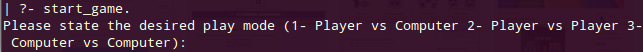
\includegraphics[scale=0.5]{startgame.png}
\caption{Menu de escolha de tipo de jogador}
\label{fig:startgame}
\end{figure}

Se o utilizador escolher um modo de jogo que envolva o computador, é depois convidado a escolher a dificuldade do bot: modo fácil ou difícil, tal como se pode ver na figura \ref{fig:botdifficulty}.

\begin{figure}[h]
\centering
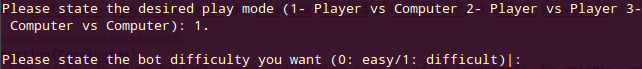
\includegraphics[scale=0.5]{botdifficulty.png}
\caption{Menu de escolha de dificuldade do bot}
\label{fig:botdifficulty}
\end{figure}

Depois, independentemente do modo escolhido, o utilizador decide se quer um tabuleiro do tipo Syrtis Major ou Syrtis Minor (figura \ref{fig:pickboard}).

\begin{figure}[h]
\centering
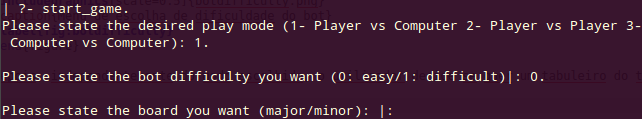
\includegraphics[scale=0.5]{pickboard.png}
\caption{Menu de escolha de tipo de tabuleiro}
\label{fig:pickboard}
\end{figure}

Depois, se o utilizador tiver escolhido um modo de jogo que envolva pelo menos um jogador, este irá escolher a posição das torres, tal como se pode ver na figura \ref{fig:picktowers}.

\begin{figure}[h]
\centering
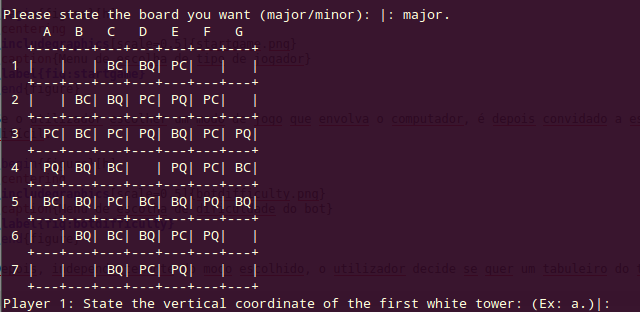
\includegraphics[scale=0.5]{picktower.png}
\caption{Menu de colocação das torres}
\label{fig:picktowers}
\end{figure}

Depois de estarem escolhidas, se o modo de jogo escolhido for jogador vs jogador, o outro jogador escolherá a sua cor. No caso de ser jogador vs computador, o computador escolherá a sua cor. Depois disso, o jogo começa. A figura \ref{fig:playtime} mostra a mensagem mostrada ao utilizador no momento da sua jogada.

\begin{figure}[h]
\centering
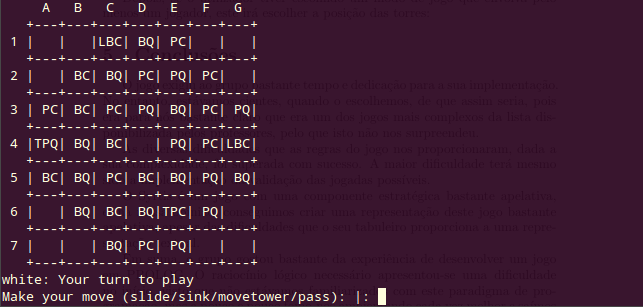
\includegraphics[scale=0.5]{playtime.png}
\caption{Menu de jogo}
\label{fig:playtime}
\end{figure}

O jogador poderá então escolher qual das 4 jogadas possíveis quer. Depois de escolhida, deverá dar as coordenadas necessárias à sua jogada, como mostrado na figura \ref{fig:playmade}.

\begin{figure}[h]
\centering
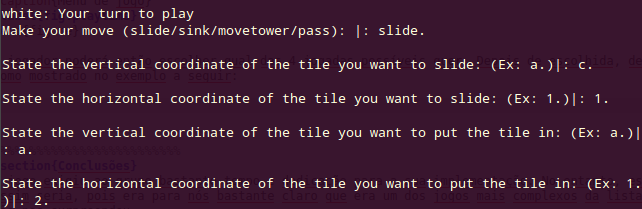
\includegraphics[scale=0.5]{playmade.png}
\caption{Jogada prestes a ser feita}
\label{fig:playmade}
\end{figure}

Depois, cada jogador (ou computador) fará sucessivamente as suas jogadas, até que eventualmente algum jogador irá ganhar. Quando isto acontece, uma mensagem é mostrada no ecrã a informar o vencedor, e o jogo acaba, tal como se pode ver na figura \ref{fig:endgame}.

\begin{figure}[h]
\centering
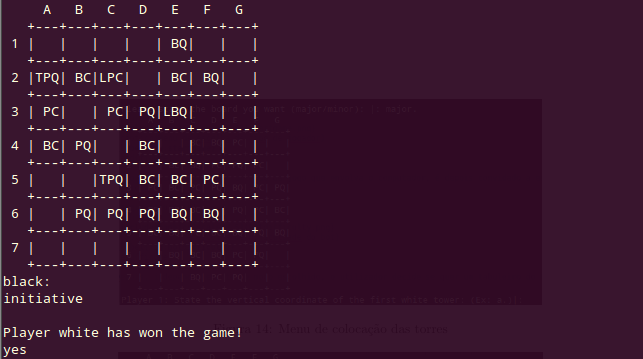
\includegraphics[scale=0.5]{gameend.jpg}
\caption{Fim do jogo}
\label{fig:endgame}
\end{figure}


%%%%%%%%%%%%%%%%%%%%%%%%%%
\newpage
\section{Conclusões}
O jogo exigiu ao grupo bastante tempo e dedicação para a sua implementação. No entanto, estávamos cientes, quando o escolhemos, de que assim seria, pois era para nós bastante claro que era um dos jogos mais complexos da lista disponibilizada pelos professores, pelo que isto não nos surpreendeu.

As diversas dificuldades que as regras do jogo nos proporcionaram, dada a sua complexidade, foi superada com sucesso. A maior dificuldade terá mesmo sido a implementação da validação das jogadas possíveis.

O Syrtis é um jogo com uma componente estratégica bastante apelativa, e, na nossa opinião, conseguimos criar uma representação deste jogo bastante apelativa, apesar das dificuldades que o seu tabuleiro proporciona a uma representação textual.

Em suma, o grupo gostou bastante da experiência de desenvolver um jogo em PROLOG. O raciocínio lógico necessário apresentou-se uma dificuldade no início, visto que não estávamos familiarizados com este paradigma de programação, mas a pouco e pouco fomo-nos ambientando cada vez melhor e saímos deste projeto definitivamente bastante mais experientes no que a ele toca.


\clearpage
\addcontentsline{toc}{section}{Bibliografia}
\renewcommand\refname{Bibliografia}
\bibliographystyle{plain}
\bibliography{myrefs}

\newpage
\appendix
\section{Código Fonte}
\lstinputlisting[language=Prolog, breaklines=true]{../board.pl}
\end{document}
